\documentclass[tikz,border=12pt]{standalone}
\usepackage[T1]{fontenc}
\usepackage{mathpazo}
\usepackage{amsmath,amssymb}
\usetikzlibrary{arrows.meta, positioning, calc}

\definecolor{stblue}{HTML}{7B97AD}
\definecolor{rwgold}{HTML}{B8995E}
\definecolor{sage}{HTML}{7A9A7E}
\definecolor{dkbrown}{HTML}{3D3530}
\definecolor{wmgray}{HTML}{7B7067}
\definecolor{cream}{HTML}{F9F6F0}
\definecolor{border}{HTML}{D4C9B8}
\definecolor{terracotta}{HTML}{C47A6A}

\begin{document}
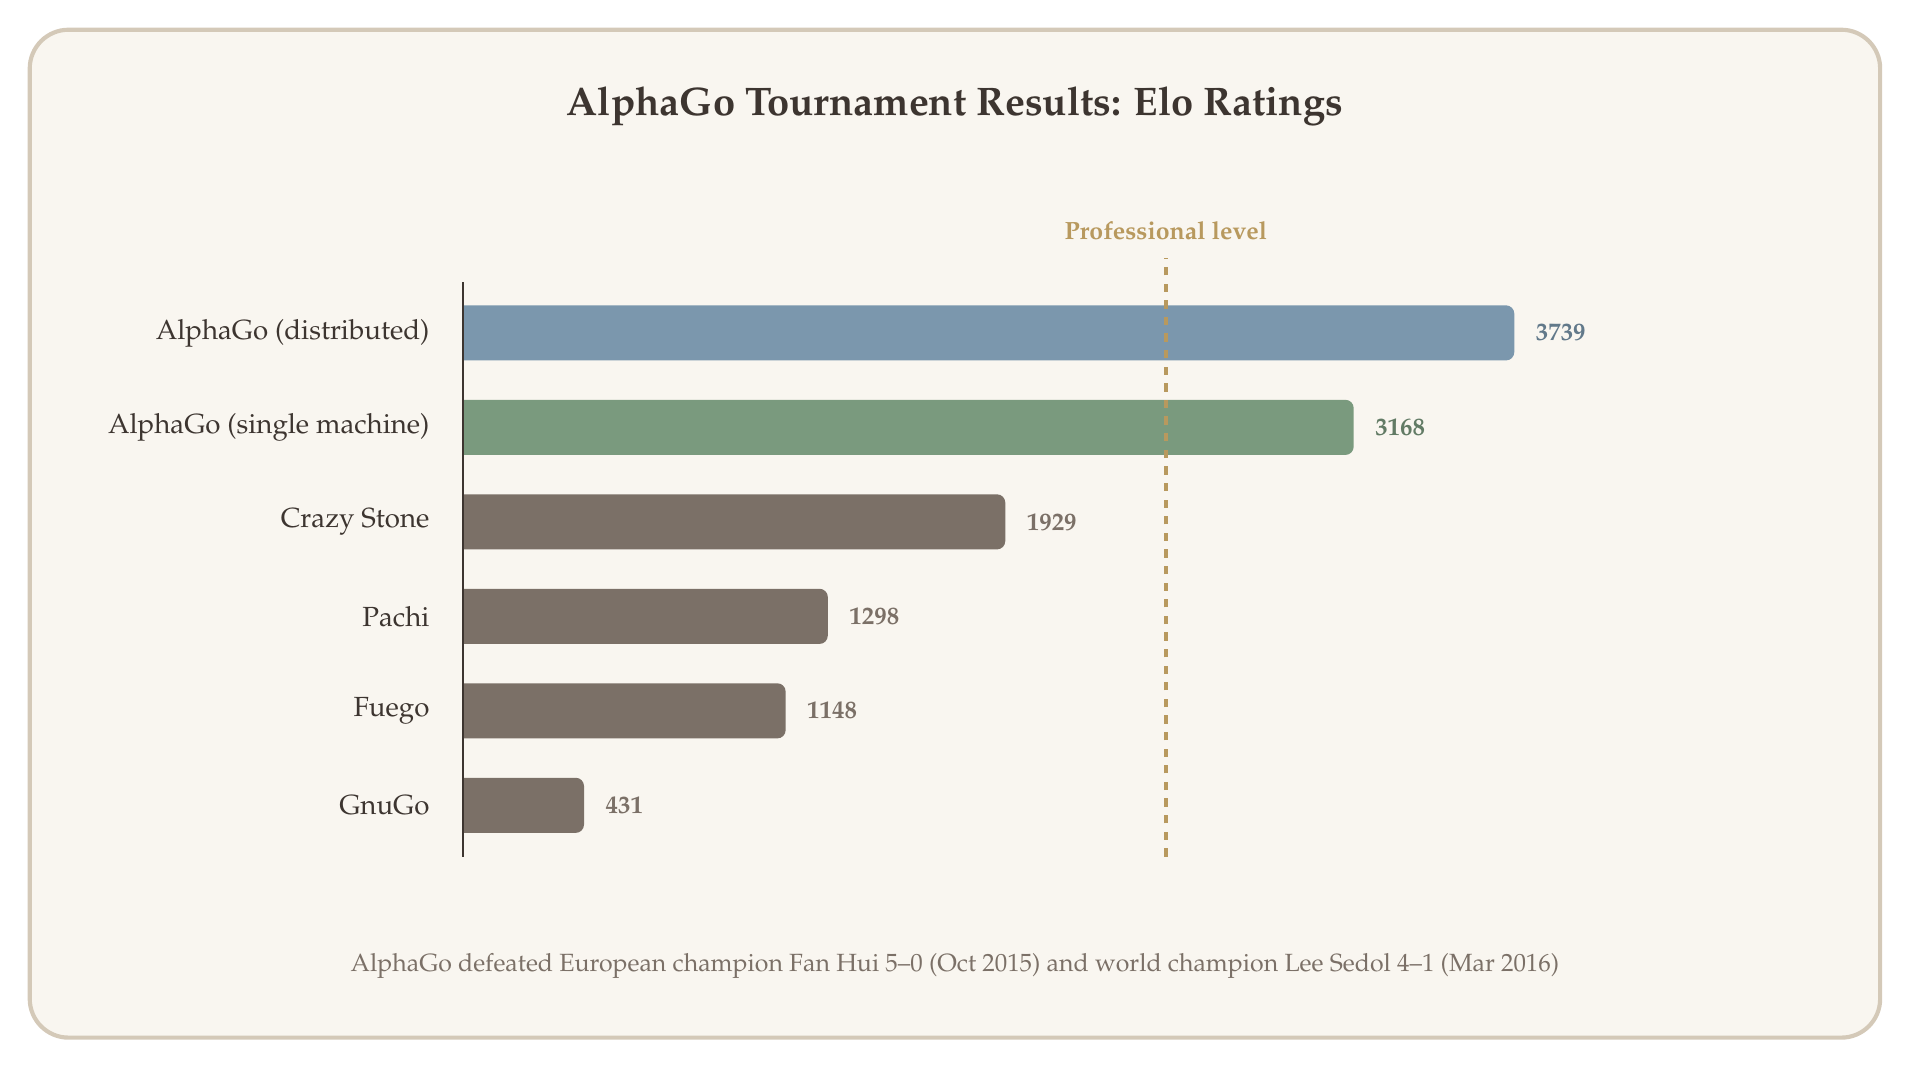
\begin{tikzpicture}[
  >={Stealth[length=3.5mm, width=2.5mm]},
]

% Dimensions
% Chart area: x from 0 to 15, y from 0 upward
% Bar height = 0.7cm, gap between bars = 0.5cm
% Total bar step = 1.2cm
% 6 bars: from y=0.6 to y=6.6

\pgfmathsetmacro{\barh}{0.7}       % bar height
\pgfmathsetmacro{\barstep}{1.2}    % vertical step between bars
\pgfmathsetmacro{\maxelo}{4200}     % x-axis max for scaling
\pgfmathsetmacro{\chartw}{15}       % chart width in cm
\pgfmathsetmacro{\labelx}{-0.3}     % right edge of label text

% Background
\fill[cream, rounded corners=14pt] (-5.5,-2) rectangle (18,10.8);
\draw[border, rounded corners=14pt, line width=1.5pt] (-5.5,-2) rectangle (18,10.8);

% Title
\node[font=\Large\bfseries, text=dkbrown, anchor=north] at (6.25,10.2)
  {AlphaGo Tournament Results: Elo Ratings};

% Data: sorted bottom (lowest) to top (highest)
% Bar 1: GnuGo 431
% Bar 2: Fuego 1148
% Bar 3: Pachi 1298
% Bar 4: Crazy Stone 1929
% Bar 5: AlphaGo (single machine) 3168
% Bar 6: AlphaGo (distributed) 3739

% Helper: bar base y
\pgfmathsetmacro{\boney}{0.6}

% --- GnuGo ---
\pgfmathsetmacro{\yy}{\boney + 0*\barstep}
\pgfmathsetmacro{\bw}{431/\maxelo*\chartw}
\fill[wmgray, rounded corners=0pt]
  (0,\yy) [rounded corners=3pt] -- (\bw,\yy) -- (\bw,\yy+\barh)
  [rounded corners=0pt] -- (0,\yy+\barh) -- cycle;
\node[font=\normalsize, text=dkbrown, anchor=east] at (\labelx, \yy+\barh/2)
  {GnuGo};
\node[font=\small\bfseries, text=wmgray, anchor=west] at (\bw+0.15, \yy+\barh/2)
  {431};

% --- Fuego ---
\pgfmathsetmacro{\yy}{\boney + 1*\barstep}
\pgfmathsetmacro{\bw}{1148/\maxelo*\chartw}
\fill[wmgray, rounded corners=0pt]
  (0,\yy) [rounded corners=3pt] -- (\bw,\yy) -- (\bw,\yy+\barh)
  [rounded corners=0pt] -- (0,\yy+\barh) -- cycle;
\node[font=\normalsize, text=dkbrown, anchor=east] at (\labelx, \yy+\barh/2)
  {Fuego};
\node[font=\small\bfseries, text=wmgray, anchor=west] at (\bw+0.15, \yy+\barh/2)
  {1148};

% --- Pachi ---
\pgfmathsetmacro{\yy}{\boney + 2*\barstep}
\pgfmathsetmacro{\bw}{1298/\maxelo*\chartw}
\fill[wmgray, rounded corners=0pt]
  (0,\yy) [rounded corners=3pt] -- (\bw,\yy) -- (\bw,\yy+\barh)
  [rounded corners=0pt] -- (0,\yy+\barh) -- cycle;
\node[font=\normalsize, text=dkbrown, anchor=east] at (\labelx, \yy+\barh/2)
  {Pachi};
\node[font=\small\bfseries, text=wmgray, anchor=west] at (\bw+0.15, \yy+\barh/2)
  {1298};

% --- Crazy Stone ---
\pgfmathsetmacro{\yy}{\boney + 3*\barstep}
\pgfmathsetmacro{\bw}{1929/\maxelo*\chartw}
\fill[wmgray, rounded corners=0pt]
  (0,\yy) [rounded corners=3pt] -- (\bw,\yy) -- (\bw,\yy+\barh)
  [rounded corners=0pt] -- (0,\yy+\barh) -- cycle;
\node[font=\normalsize, text=dkbrown, anchor=east] at (\labelx, \yy+\barh/2)
  {Crazy Stone};
\node[font=\small\bfseries, text=wmgray, anchor=west] at (\bw+0.15, \yy+\barh/2)
  {1929};

% --- AlphaGo (single machine) ---
\pgfmathsetmacro{\yy}{\boney + 4*\barstep}
\pgfmathsetmacro{\bw}{3168/\maxelo*\chartw}
\fill[sage, rounded corners=0pt]
  (0,\yy) [rounded corners=3pt] -- (\bw,\yy) -- (\bw,\yy+\barh)
  [rounded corners=0pt] -- (0,\yy+\barh) -- cycle;
\node[font=\normalsize, text=dkbrown, anchor=east] at (\labelx, \yy+\barh/2)
  {AlphaGo (single machine)};
\node[font=\small\bfseries, text=sage!80!black, anchor=west] at (\bw+0.15, \yy+\barh/2)
  {3168};

% --- AlphaGo (distributed) ---
\pgfmathsetmacro{\yy}{\boney + 5*\barstep}
\pgfmathsetmacro{\bw}{3739/\maxelo*\chartw}
\fill[stblue, rounded corners=0pt]
  (0,\yy) [rounded corners=3pt] -- (\bw,\yy) -- (\bw,\yy+\barh)
  [rounded corners=0pt] -- (0,\yy+\barh) -- cycle;
\node[font=\normalsize, text=dkbrown, anchor=east] at (\labelx, \yy+\barh/2)
  {AlphaGo (distributed)};
\node[font=\small\bfseries, text=stblue!80!black, anchor=west] at (\bw+0.15, \yy+\barh/2)
  {3739};

% --- Vertical baseline at x=0 ---
\draw[dkbrown, line width=0.8pt] (0,0.3) -- (0,\boney + 5*\barstep + \barh + 0.3);

% --- Professional level dashed line at Elo 2500 ---
\pgfmathsetmacro{\profx}{2500/\maxelo*\chartw}
\draw[rwgold, line width=1.5pt, dashed]
  (\profx,0.3) -- (\profx,\boney + 5*\barstep + \barh + 0.6);
\node[font=\small\bfseries, text=rwgold, anchor=south]
  at (\profx, \boney + 5*\barstep + \barh + 0.7)
  {Professional level};

% --- Bottom annotation ---
\node[font=\small, text=wmgray, anchor=north, align=center] at (6.25,-0.8)
  {AlphaGo defeated European champion Fan Hui 5--0 (Oct 2015)
   and world champion Lee Sedol 4--1 (Mar 2016)};

\end{tikzpicture}
\end{document}
